\documentclass{acm_proc_article-sp}
\usepackage{amsmath}
\usepackage{algorithm}
\usepackage{algpseudocode}
\usepackage{multirow}
\usepackage{bbold}

\renewcommand{\algorithmicrequire}{\textbf{input: }}
\renewcommand{\algorithmicensure}{\textbf{output: }}
\newcommand{\mr}[1]{{\it MR: {\small #1}}}
\newcommand{\eat}[1]{}

\begin{document}

\title{How stories evolve: News graphs as a way to represent context and evolution of news stories}

\numberofauthors{1} %  in this sample file, there are a *total*
% of EIGHT authors. SIX appear on the 'first-page' (for formatting
% reasons) and the remaining two appear in the \additionalauthors section.
%
\author{
%
% 1st. author
%\alignauthor 
%Rahul Goyal, Ravee Malla, Amitabha Bagchi, Sameep Mehta, Maya Ramanath\\
%  \affaddr{Indian Institute of Technology}\\
%  \affaddr{New Delhi, India}\\
%  \email{\{rahulgoyal34, ravmalla\}@gmail.com, \{bagchi, ramanath\}@cse.iitd.ernet.in}
% 2nd author
%\alignauthor 
%Author 2\\
  %\affaddr{Research India}\\
 % \affaddr{New Delhi, India}\\
 % \email{author2@in.ibm.com}
}

%\date{25 March 2013}

\maketitle
\begin{abstract}
Providing the history and context(s) of a news article that emerges in
the middle of an evolving news story--sometimes multiple news stories--is
a complex task. The complexity of the task is compounded by the fact that
different users are interested in different contexts of the article, and
it is impossible to guess what a particular user is most interested in. In
this paper, we introduce ESTHETE, a system that provides rich context(s)
(through what we call {\em personalized flexible context
extraction}), by preprocessing and storing articles in a structured
representation (directed graphs) that makes it easy for the user to
explore different contexts. We formally define what constitutes a ``good'' news story and give an algorithm
to efficiently compute coherent and contextfull news stories from the news graph. The advantage of this approach is that the
incremental computational expense in incorporating new articles as they are published is minimal.
We describe the design and features of ESTHETE, and present the results of a comprehensive user study highlighting the usefulness of our system. 
Our system is available at: {\tt http://konfrap.com/esthete}.

\end{abstract}

%{\bf MR: Abstract can be made tighter}

% A category with the (minimum) three required fields
\category{H.4}{Information Systems Applications}{Miscellaneous}
%A category including the fourth, optional field follows...
%\category{D.2.8}{Software Engineering}[performance measures]

\terms{News Corpus Visualization, Flexible Personalized Context-rich News graph, News Summarization, System for News browsing, Interface Design}

%\keywords{ACM proceedings, \LaTeX, text tagging} % NOT required for Proceedings

\section{Introduction}
Online news websites are now a common way of consuming news. These
websites are very helpful in publishing breaking news and help users
keep up to date with the latest developments. However, the
proliferation of these websites simply means that we are drowning in
more news than we know what to do with. Specific news stories that we
would like to follow over days or weeks may be buried among more
current or recent news. Navigating through a maze of articles looking
for ones of interest is a non-trivial task.  

Current news websites do not do much to help users trace the origin of
these stories, nor how they overlap with each other. Most of them
still ``look'' like news papers with a bunch of articles laid out on
the web-page, with a few additional features in the form of ``Related
News'' and ``Recommended News'' links. A reader trying to
contextualize a particular article can follow some of these links but
the context provided by these features is shallow and tracing the
development of the story with its various aspects is not much easier
than it was in the days of paper-based news media. The news corpus is
available in electronic form, carefully archived by all news
organizations. There have been some recent efforts by the research
community that attempt to extract individual strands of a stories
development from the corpus~\cite{shahaf@kdd2010} or present
interacting strands in a mesh-like
structure~\cite{shahaf@www2012}. Still others use graph-like
abstractions, just like we do, to approach the limited problem of
detecting a news item that represents the development of a news
story~\cite{subasic-icdm:2008,subasic-ida:2013}. What remains missing
is the structural framework required to process it into a form that
would make it possible for a user to elaborate the many contexts
behind a single news story, some stretching years into the past, some
just a few days. 

To make this concrete let us consider the unfortunate gang-rape
incident that took place in Delhi in December 2012. Since the day this
crime was first reported by the media, it grew into a complex news
story, talking about related rape cases of the past, the reactions of
various sections of the society (politicians, activists, human rights
organizations, etc), the health of the victim up to her tragic death,
the investigation carried out by the law enforcement authorities and
the judicial proceedings against the offenders once they were
caught. Different users may want to focus on different aspects of this
story. For eg., consider a graph of news articles around this story
shown in Figure~\ref{fig:context-adding-graph-gang-rape-1}.  We see
three of the many possible contexts that can be followed and utilized
by a user to better understand the overall picture. We allow the user
to express her intent to follow a particular context (either ``the
reactions of Politicians'' or ``the victim's condition'' or ``the
Police investigations'') and understand the story with that
context. This results in a view that is personalized for a particular
user, since she is free to choose the context(s) that help her follow
the story. We call this notion \emph{Personalized Flexible Context
  Extraction}. This notion is an extremely natural approach that a news
consumer, whether an expert commentator or a lay person, might want to
employ as a crucial subtask in the process of news consumption. We
believe that it is possible to realize this notion given the
development in information extraction techniques that has taken place
in the last few years. However this realization requires the
specification and implementation of a  framework for
(pre)processing and structuring the news corpus in such a way that it
can easily serve information needs that cannot always be forseen when
the news emerges.

\begin{figure}[ht]
\caption{How multiple contexts are added to a single story}
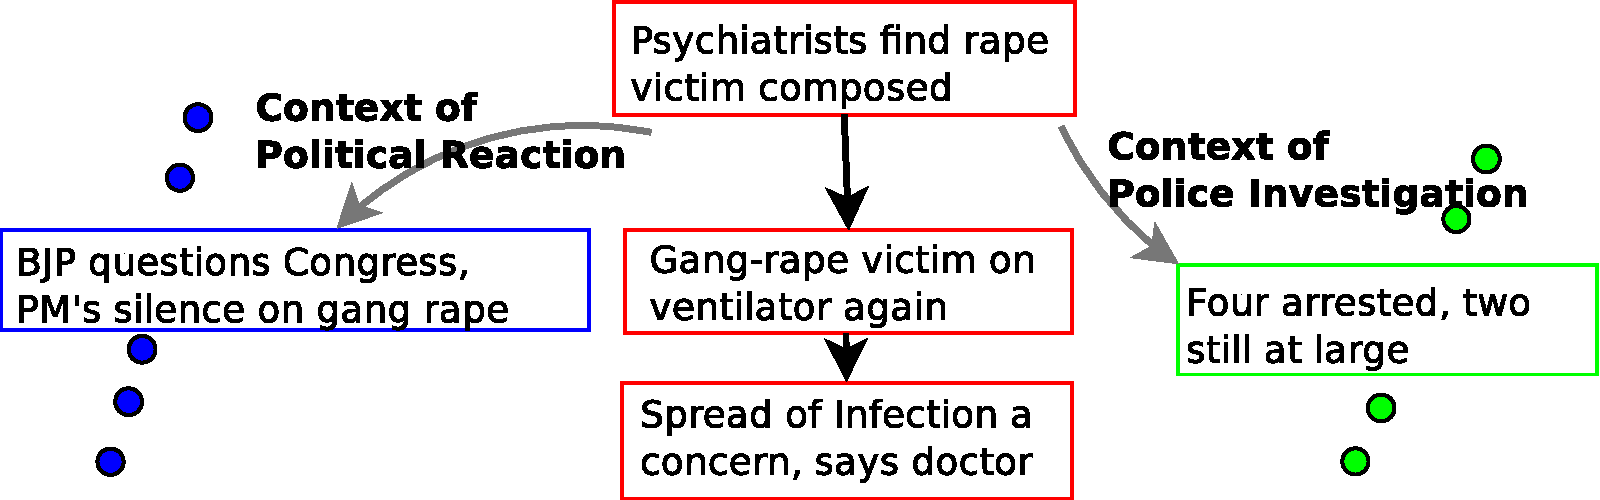
\includegraphics[scale=0.31]{figures/graph-3.pdf}
\label{fig:context-adding-graph-gang-rape-1}
\end{figure}


%What we want to do about it -- this paragraph is pretty weak
Our attempt in this paper is to provide such a framework and show that
it can be used in a flexible way by a user to fulfill his or her need
to contextualize what he or she is reading in the news.  Building on
the work of~\cite{choudhary@ecir2008} that models news corpora as a
time-evolving graph by linking related news articles, we provide a
query mechanism that organizes this structure by topics of interest
and important actors, and presents the development of a story on a
timeline. The user can now interact with the result by filtering
articles based on topic, entities, time, or a combination of all
three. For example, Figure~\ref{fig:complete-tool-screenshot} shows
the timeline of the recent rape case incidents reported from India.

An important aspect of our work that represents a completely different
approach from the prominent attempts at news corpus processing and
extraction in the literature is that we take an offline approach
i.e. we view the news corpus as an evolving entity that is streaming
past us. We store it in a structured way such that it can be browsed
and, importantly, {\em different kinds of contexts can be extracted
  from it by users with different approaches to the same news
  stories}. This represents a break in thinking from those approaches
that take the entire news corpus as their input and either produce an
output which {\em is} the story~\cite{shahaf@kdd2010,shahaf@www2012}
or produce some output based on a pre-existing notion of what is the
story~\cite{subasic-icdm:2008,subasic-ida:2013}. We allow the user to
build the story. Apart from providing lower flexibility to the user,
in our opinion, these other approaches are fundamentally not-scalable
since every time an information need arises a set of expensive
computations has to be done. Our approach can be thought of as a
data-structuring approach: We preprocess the data to make news
browsing and user-led context discovery an easier and computationally
feasible process.

%Contributions
In summary, our contributions are as follows:
\squishlist
\item We build on a graph-based framework (\cite{choudhary@ecir2008}) to represent articles in a news corpus and make it query-able. 
\item We propose metrics to capture utility of a news article to understand a news story in terms of the coherent context provided by it.
\item We propose an efficient graph-based algorithm to find useful contexts around a news story that help to get the bigger picture.
\item We provide an interactive interface to users which is easy to use, and helps in tracking the evolution of the story and zooming
  to specific parts of interest.
\item We report on the results of a thorough evaluation of our system and show that our system compares well with existing ones.
\squishend

\textbf{Organization:} The rest of the paper is organized as
follows. We first summarize the related work that has addressed the
problem of news corpus mining, categorizing it under various threads
(Section~\ref{sec:related}). We then formally state our definition of
a personalized flexible context extracting news browsing tool,
describing the basic features of such a tool and our approach to
building such a tool based on the news graphs
of~\cite{choudhary@ecir2008} (Section~\ref{sec:newsgraph}).  In
particular, we introduce the notion and importance of \emph{context}
of this news graph, and describe how these contexts can be extracted.
Next, we give a detailed block-by-block description of our system
(Section~\ref{sec:block}). We then present results from various
evaluation experiments conducted on our news browsing system
(Section~\ref{sec:eval}). Finally, we conclude with some
observations and future scope (Section~\ref{sec:conclusions}).

\section{Past Work}
\label{sec:related}

Our works builds upon several areas of research, in particular the graphical representation of news articles, the identification and tracking of topics, time-based story and event evolution, multi document summarization, and information visualisation.

\paragraph*{Graph representation of Articles} Choudhary et al.\cite{choudhary@ecir2008} proposed (which was at that time) a novel method of organizing a news corpus into a directed graph, by mining and tracking the \emph{transformations} that the entities in the corpus undergo. These transformations, defined for one or more entities, can be one of the following:
\squishlist
  \item \textbf{Birth:} An entity appearing for the first time
  \item \textbf{Cease:} An entity appearing for the last time
  \item \textbf{Merge:} Two entities co-occurring for the first time
  \item \textbf{Split:} Two entities co-occurring for the last time
  \item \textbf{Continue:} An entity remaining popular in a period
\squishend
Their idea can be summarized as follows: 1) Mine transformations in the article set 2) Find a weighted-edge covering of all transformations.
For a more detailed description, we refer the reader to the paper. The work does not discuss how such a news graph may be mined to extract
useful information, rather proposes this graph as a means of visualizing the news. However, such graphs easily blow up as the complexity
of the news story increases. 

Figure~\ref{fig:sample-news-graph} shows an example graph that gets created using this technique for a set of 4
articles covering a crime story. Nodes $A$ and $B$ talk about the incident being reported, reactions from various sections of the society and
the progress of investigation. Then, there is a fork in the story, with node $C$ talking about the fate of the investigating officer Damayanti Sen, 
and node $D$ talks covers the judicial probe of the incident. The nodes $C$ and $D$ cover different different aspects of the same story.
\begin{figure}
\caption{A news graph of a crime incident from Bengal}
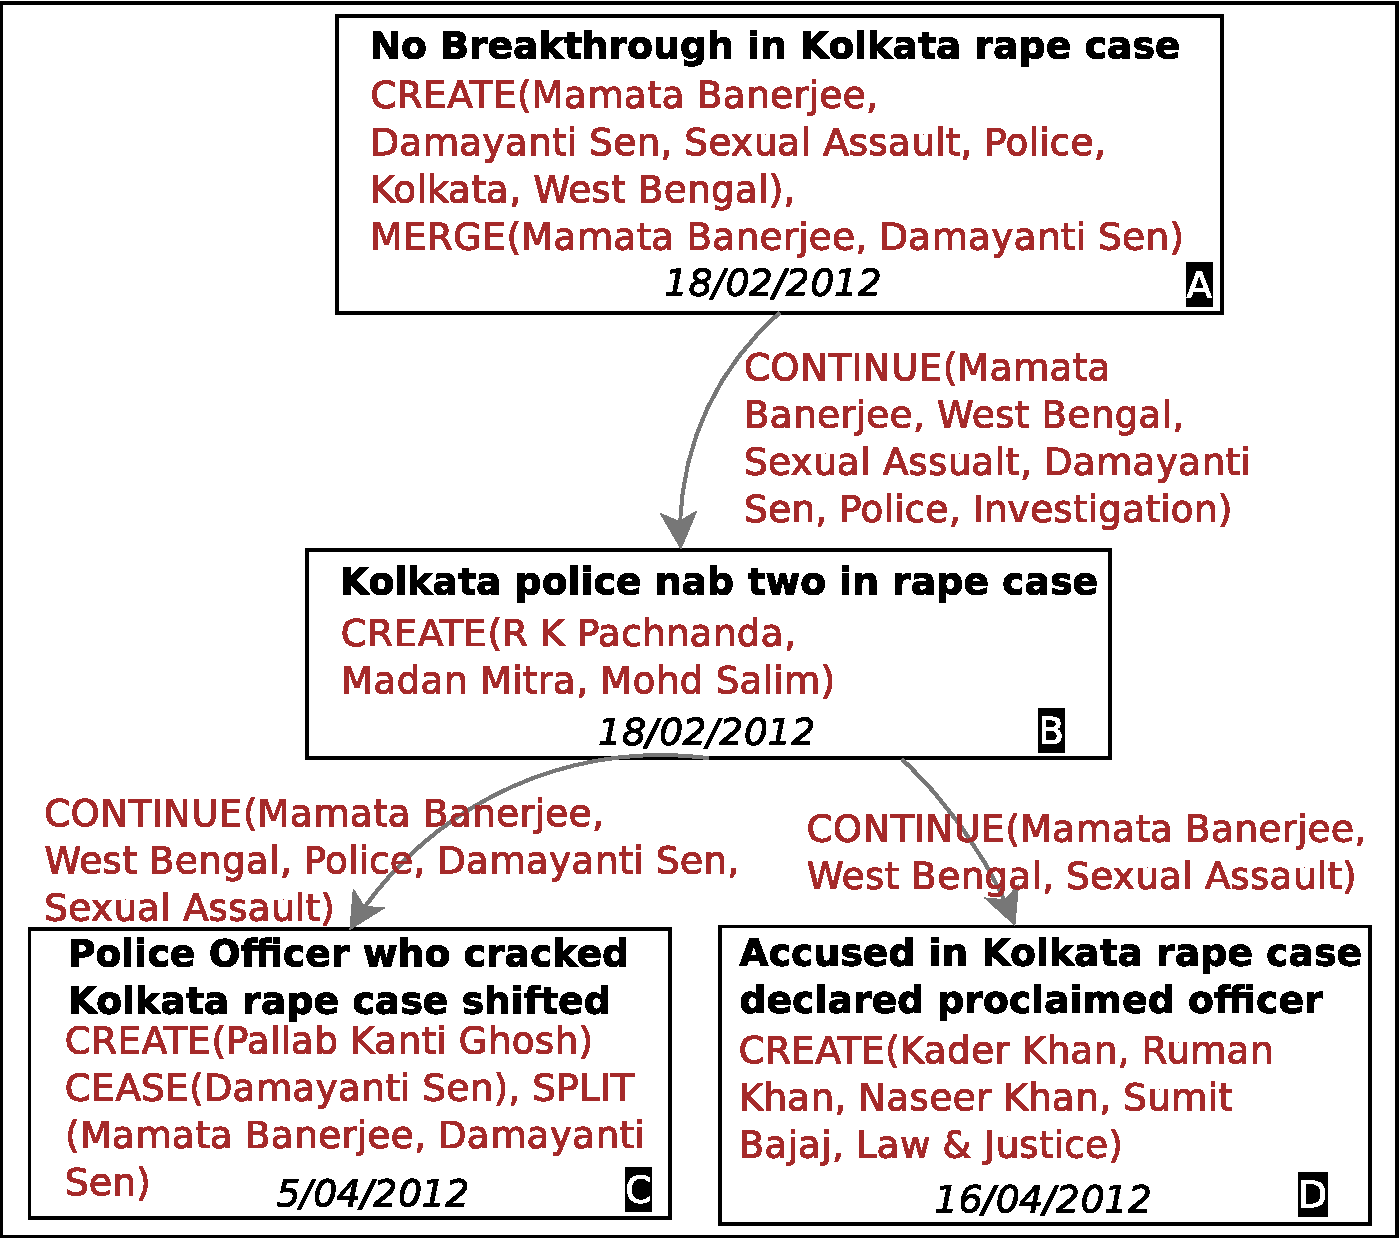
\includegraphics[scale=0.36]{figures/graph-1.pdf}
\label{fig:sample-news-graph}
\end{figure}
\paragraph*{Topic Detection and Tracking} Topic Detection \& Tracking (TDT) is a well studied problem \cite{springerlink:10.1023/B:INRT.0000011210.12953.86, springerlink:10.1007, Franz:2001:USC:383952.384013}. In TDT, a topic is defined as a collection of important words by considering documents to be bags-of-words. In ``Topic detection'', one determines clusters of articles that discuss the same topic, while in ``Topic tracking'', one detects stories that discuss a previously known topic \cite{Allan:2002:TDT:772260}. 

\paragraph*{Story Evolution}  Kim et al.\cite{Kim:2011:TCU:1964750.1964765} propose a method for detecting and tracking latent topics that appear within news articles, and visualize how the news corpus evolves from one topic set to another using topic similarity metrics. Suba\v{s}i\'{c} et al.\cite{subasic-ida:2013} %CONFIRM THIS IS THE RIGHT REFERENCE
 show how an event emerges, changes and disappears by dividing each event into several time stages and forming a network of co-occurence of terms based on frequency and time relevance. Nallapati et al.\cite
{Nallapati:2004:ETW:1031171.1031258, Mei:2005:DET:1081870.1081895} present a system to discover subtopics within a news topic and construct a graph showing their inter-dependencies. These systems are best-suited for simple linear news stories and may not work well for complex stories. In an extension to their previous work \cite{shahaf@kdd2010}, which finds the most coherent chain of articles that cover the story connecting 2 input articles, Shahaf et al.\cite{shahaf@www2012} construct a roadmap of chains of stories, which may have many branches of smaller stories. 

\paragraph*{Summarization} Barzilay et al.\cite{Barzilay:2002:ISS:1622810.1622812} talk about multidocument news summarization to generate a coherent and comprehensive summary from an input sequence of articles.

\paragraph*{Visualization} Vydiswaran et al.\cite{MEET:MEET14504801078} design a system to explore news by querying for topics, time range and locations. However, they process articles per user query. In addition, there is no notion of tracking news evolution on a timeline.

As far as we know, our work is the first attempt towards using a rich graph structure built out of the raw articles, that is amenable to repetitive querying without any significant cost of post-processing. Having such a structure, allows us to run efficient algorithms on the news article stream to mine and track the underlying news stories and to provide a personalised context to the story tailored to the user's query. Further, by visualizing these stories on a timeline, it helps the user follow the progression of the story through the different actors and topics.

\section{The news browsing problem}
\label{sec:newsgraph}

Our problem statement can be formally stated as:
\begin{quote}
  Create an end-to-end news browsing system which given a
  continuous stream of raw news articles, processes these articles to
  mine and track the underlying news stories and visualizes these for
  a user on an easy-to-use, queryable, personalized and context-full
  interface.
\end{quote}
As discussed in the previous section, various approaches have been proposed in the past to tackle one or more components of the above problem
statement. In this section, we first define a notion of contextuality of a browsing system, and motivate the need for the system to serve multiple flexible and personalizable contexts to a user as per her
requirements and/or preferences. We reason why we think this is a necessary feature of a news browsing system. Next, we show how rich contexts can be served to a user on the fly based on her intent
from the graph structure created from the input news corpus, taking specific examples. 
Finally, we describe some other desirable features of a news browsing tool. 

\subsection{Context in News browsing}
Let us attempt to define clearly what we mean by context. The
dictionary definition of the word is ``the circumstances that form the
setting for an event, statement or idea, and in terms of which it can
be fully understood and assessed.'' But the term ``circumstances'' is
vague and does not help us. So, instead, viewing the news corpus as a
time indexed set, we can think of the following definition: 
\begin{quote}
Given a news article or articles (from here on, referred to as our result set), {\em context} is that set of stories
preceding, co-occuring or following that article or articles which
enhance our understanding of the events or ideas described in that
article or articles.
\end{quote}

Context for a user using our system, comprises of articles, topics,
actors, events, etc which though not directly related to particular
story, helps to interpret the story in a broader sense.  Adding
context serves to make it easier for users to better understand chain
of news articles around an event. For eg., consider a crime story
where the prime suspect is $X$. To fully understand the involvement of $X$ in the story,
one may be required to go through articles which would have first reported the crime (and not 
mentioned $X$). These articles serve as context. Hence, one way to think of context-serving articles
are \emph{articles which are coherent with articles containing $X$ and have still more information to provide.}

Given this intuition, we now propose a natural algorithm to determine useful context for a particular part of
the news graph in consideration. Say a user, on a certain filter query, is presented with an article $a$. We want to identify articles
conntected to $a$ via a path in the graph, which would be helpful to the user to understand the story and the bigger picture.

We first define the notion of Continue strength $\Omega$ of an actor at some time, which captures an actor's popularity in at that time.
Let $\Lambda$ be the set of all actors, $T$ the time index set, then $\Omega : \Lambda \times T \rightarrow [0,1]$. This score is aggregated over all the articles featuring this actor.
\begin{equation}
\Omega(\lambda, \tau) = \frac{\sum_{a \in A([\tau - P, \tau + F])}{ContinueScore(\lambda, a, \tau)}}{|A([\tau - P, \tau + F])|}
\end{equation}
Here, $ContinueScore(\lambda, a, \tau)$ is the continue score (as defined in \cite{choudhary@ecir2008}) of an actor $\lambda$ occurring in article $a$ published around the current time point $\tau$. 
\begin{equation}
ContinueScore(\lambda, a, \tau) = \frac{\sum_{a \in A([\tau - P, \tau + F])}\mathbb{1}(\lambda \in a)}{|A([\tau - P, \tau + F])|}
\end{equation}
This score is normalized between 0 to 1. $P$ and $F$ are past and future time windows that we keep at 50 days each, and $A([\tau - P, \tau + F])$ are all the articles in this time window.

Now, we define the following 3 metrics to help us decide whether article $b$ should be served to the user alongside article $a$.
\begin{enumerate}
\item $coh_a(b)$: Coherence of article $b$ with article $a$
\item $cont_a(b)$: Context added by $b$ to $a$ 
\item $r(a, b)$: Weight of the edge joining node $a$ and $b$.
\end{enumerate}

\subsubsection*{Coherence}
Given an article $a$, we define $coh_{a}(b)$ as the \emph{coherence} between $a$ and some another article $b$. Intuitively, coherence captures the continuity of story when the two articles are read in succession.
Clearly, coherence between 2 articles depends on the amount of their actor/topic overlap. Moreover, common actors with strong continue scores should contribute less to coherence. This is because a strong continue score reflects the strong presence (lower importance) of the actor in articles in that particular time window. So, we quantify coherence as
\begin{equation}
coh_{a}(b) = \frac{\sum_{\lambda \in E(a) \cap E(b)}{\Omega(\lambda, \tau)^{-1}}}{|E(a) \cup E(b)|}
\end{equation}
where $E(a)$ is the set of actors occurring in article $a$ and $\tau$ is the time at which article $a$ is published. 

\subsubsection*{Context}
Along the same lines, we define $cont_{a}(b)$ as the \emph{context} given by an article $b$ to $a$. There are two different kinds of context that a user may be interested in: 1) Context provided by different actors/topics and how they relate
to the story in $a$. For instance, for the Delhi gang rape story, articles related to the rape incident that happened in Kolkata and controversy surrounding it provide this type of context. 2) Context of the same actors/topics in a slightly different setting. For instance, for the October 2012 petrol price hike story, articles related to the price hike from May 2012 provide this type of context. Context added by an article $b$ can be quantified by the degree of ``new information'' added by $b$.
So, we compute context as
\begin{equation}
cont_{a}(b) = \frac{\sum_{\lambda \in E(b)}{\Omega(\lambda, \tau)*ContinueScore(\lambda, a)^{k}}}{|E(b) - E(a)|}
\end{equation}
where $k \in [-0.5, 0.5]$ is a user-input parameter which influences which of the 2 kinds of context is more prominent. A higher $k$ prefers context having more information
around the same actors as those of our article of interest. For our experiments, we have kept the value of $k$ as 0.

\subsubsection*{Edge weights}
\cite{choudhary@ecir2008} defined the edge weight $r:V \times V \rightarrow [0,1]$ as:
\begin{equation}
r(a, b) = sim(a,b) * Jacc(E(a), E(b)) * e^{-\alpha(\tau_a - \tau_b)}
\end{equation}
Here, $sim$ is cosine similarity between articles represented as vectors in the TfIdf space, $Jacc$ is the jaccard similarity between
the entity sets of articles $a$ and $b$, and the final term is to factor in the time elapsed between their publishing dates ($\tau_a$ \& $\tau_b$).

Next, we normalize these metrics between 0 to 1 by dividing with the maximum score that is observed in the window defined by $(\tau - P, \tau + F)$. This
step is needed so we can compare these scores across different news stories. Our cumulative score is the product of these metrics.

Finally, we apply the following algorithm to get the ``most useful'' neighbourhood of the articles that are the result of user's filter query. This algorithm is a walk on the news graph starting from every article $a$, 
going as far as the cumulative score does not drop below a threshold $\theta$.

\begin{algorithmic}
  \State \textbf{\underline{GetNeighbourhood}}
  \State \algorithmicrequire{Node $n$, Current Weight $w$, Threshold $\theta$}
  \State \algorithmicensure{Neighbourhood $N$}
    \If {$w < \theta$}
      \State return \{\}
    \EndIf
    \State $N = N\cup\{n\}$
    \ForAll{node $v \in EdgeSet(n)$}
      \If {visited($v$) == False} 
        \State visited($v$) = True
        \State $w_1 \leftarrow coh_{n}(v)$
        \State $w_2 \leftarrow cont_{n}(v)$
        \State $w_3 \leftarrow r(n,v)$
        \State $w_{eff} \leftarrow w_1 * w_2 * w_3 * w$
        \State GetNeighbourhood($v, w_{eff}, \theta$)
      \EndIf
    \EndFor
\end{algorithmic}

Here, $EdgeSet$ returns all of a node's neighbours that are not covered in the result set. We initialized the neighbourhood set $N$ as an empty
set, and kept $\theta=0.5$ for our experiments.  We now give some examples of context in the news graph.

\begin{figure}
\caption{Robert Vadra corruption story and its contexts}
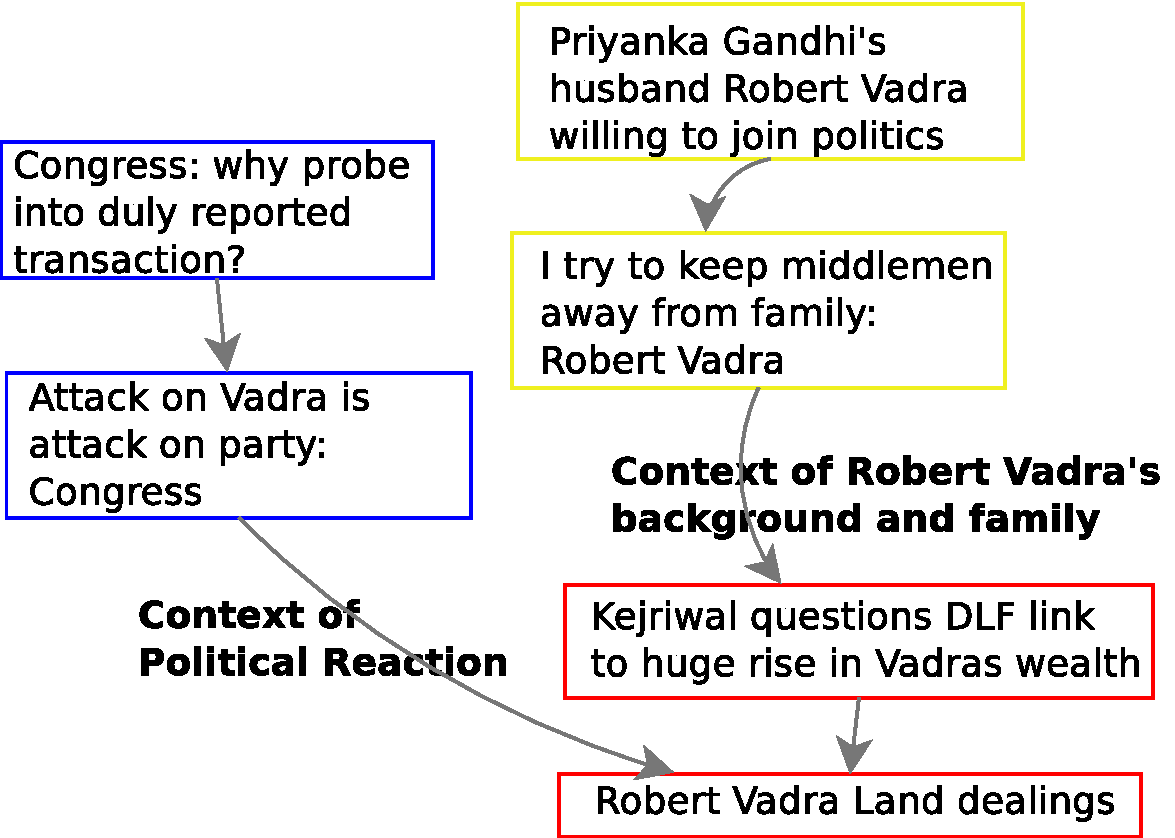
\includegraphics[scale=0.36]{figures/graph-vadra.pdf}
\label{fig:vadra-corruption}
\end{figure}

Consider Figure~\ref{fig:vadra-corruption} showing the graph of the story around Robert Vadra's alleged
corruption scandal reported in the news. As the story progresses in time, the articles
start to assume that the reader has enough knowledge of who Robert Vadra is, what is he known for,
how has this controversy spiralled to include the top political parties of India, etc. Hence, these articles
become increasingly inaccessible to a user with less prior context. However, 
using the graph, we can provide this context at any stage. Moreover, while following the story, 
the reader can look for how have the political parties reacted to this story as another context.

\begin{figure}
\caption{The fuel price hike story (September 2012) and its contexts}
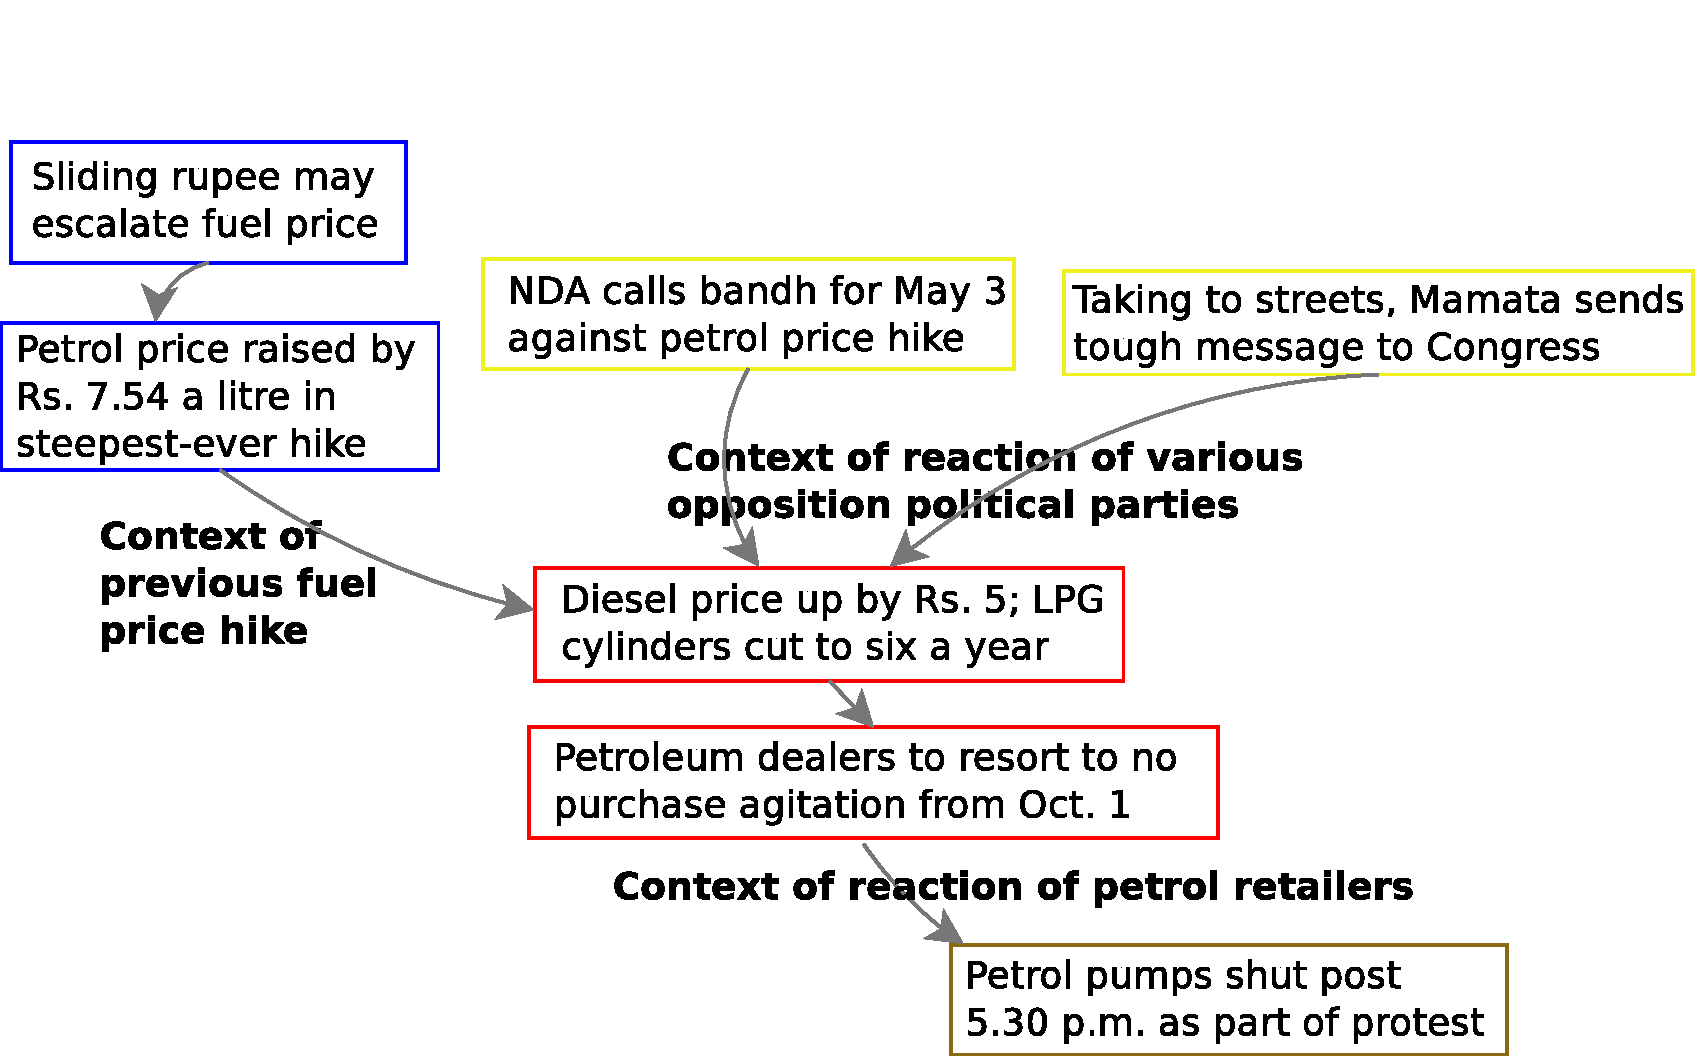
\includegraphics[scale=0.32]{figures/graph-petrol.pdf}
\label{fig:petrol}
\end{figure}

As a final example, consider the Figure~\ref{fig:petrol} showing the graph of the articles talking
about the Indian government's decision to raise the fuel price, and its past and subsequent developments. 
For a user wanting to deeply understand the circumstances behind fuel price hikes in India, the context of 
all past fuel price hikes is vital. For other users, the political
sphere and its reactions or the reactions of the petrol retailers may be of more interest.

As we have seen context is a fairly general notion and can be
instantiated in many ways depending on the user's point of view. It is
also clear from the examples above that the primary mode of inferring
contextual relationships between articles is by studying the
co-occurence and development of relationships of actors and topics in
time. We now discuss the {\em news graph} first defined
in~\cite{choudhary@ecir2008}, which provides a natural representation
of such relationships.


\subsection{How the news graph of~\cite{choudhary@ecir2008} creates personalized contexts}
Using the graph, the users have access to multiple contexts which
develop a unique aspect of the story they are following, and which
could highlight and bring forth previously unknown connections among
actors and topics. In this section, we will take examples to show how
different users would want/choose to explore same/different contexts
of the same story they are studying.

Consider two different users, both of whom want to study the Delhi gang-rape story visualized in Figure~\ref{fig:context-adding-graph-gang-rape-1}. However, when presented
one of the users wishes to study the reactions of politicians in depth, while the other wants to analyze the response and effectiveness of the police
machinery. Both these users will focus on different contexts, and soon personalize the base graph by filtering on it appropriate to their information
requirement. As a system, we never took any rigid decision to call only some of the related nodes as the ``most appropriate context''. This allows
the user to look through multiple other contexts, and then have the flexibility to choose the one that interests them the most. Moreover, this context
is calculated on the fly subject what part of the graph is in focus at that instant. As the users move across in the graph, the contexts for them keep
changing, and we can track these contexts efficiently using the graph structure.

Consider Figure~\ref{fig:context-graph-example} where 3 distinct stories are presented. The nodes marked $A$(in blue) cover a case involving Dominique Strauss-Kahn (DSK), 
those marked $B$(in red) cover of a case surrounding Pascal Mazurier(PM), and those marked $C$(in green) talk of the internationally reported Gang-rape case
that happened in Delhi(DGR).\footnote{Kindly note that in no way do we want to use this unfortunate incident or others used in the paper in any way except 
to exemplify the technicalities of our work. As reported in \cite{subasic-icdm:2008}, it is unfortunate that negative incidents are highlighted in the media
with greater vociferousness.} Two key things can be noted here. Even with a fair overlap of topics (Sexual Assault, Rape), the DSK and DGR subgraphs are not directly linked to each other.
On the other hand, the PM and DSK stories have a direct link in between them. This points to the fact, that the graph algorithm is successfully able
to determine how close or far stories (subgraphs) are to each other. Moreover, for any subgraph, one can define the \emph{context-giving node} as 
a neighbour which when shown to the user, would make it easier for her to understand the story and put in a broader perspective. For eg., if someone
wants to know about Ram Singh, the prime accused in the DGR case, just looking at the articles featuring Ram Singh won't suffice, since he would be
discussed in other articles where his name won't have featured explicitly (as he is still on the run). Such context-giving nodes are shown in bold outline in the figure.

Figure~\ref{fig:sample-news-graph} shows an example graph that gets created for a set of 4
articles covering a crime story. Nodes $A$ and $B$ talk about the incident being reported, reactions from various sections of the society and
the progress of investigation. Then, there is a fork in the story, with node $C$ talking about the fate of the investigating officer Damayanti Sen, 
and node $D$ talks covers the judicial probe of the incident. The nodes $C$ and $D$ cover different different aspects of the same story. 
\begin{figure}
\caption{A news graph of a crime incident from Bengal}
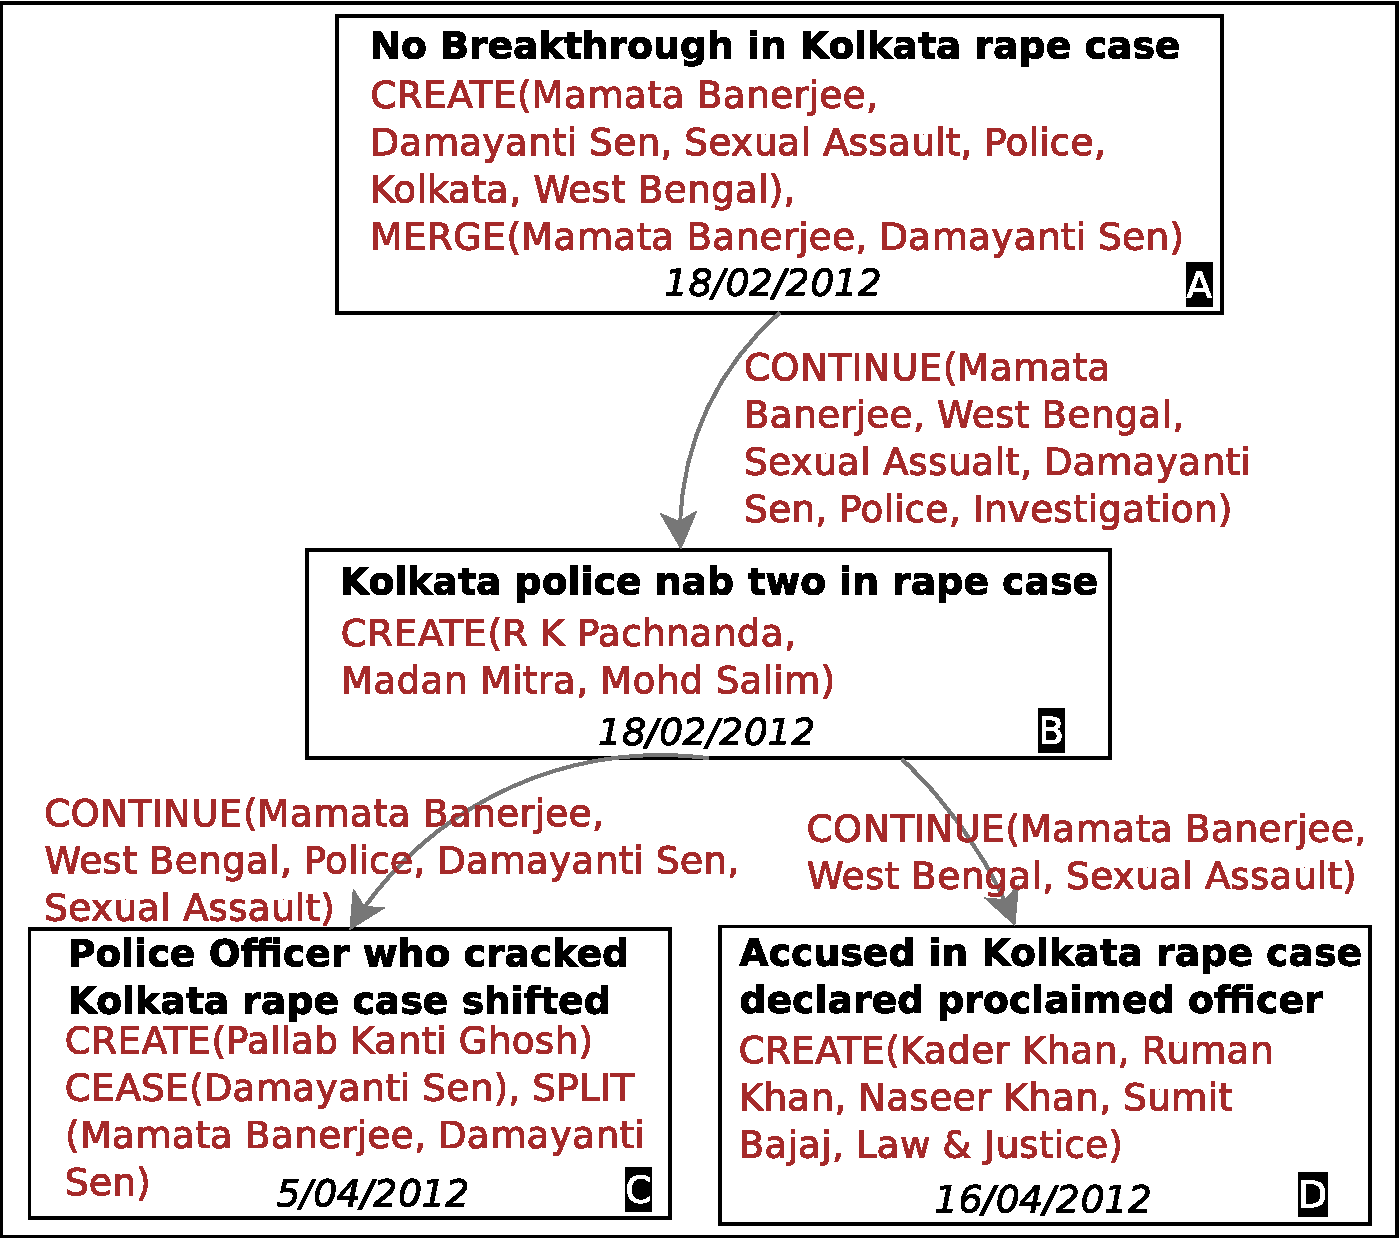
\includegraphics[scale=0.36]{figures/graph-1.pdf}
\label{fig:sample-news-graph}
\end{figure}
A key strength of our approach is that we allow the user to iteratively query the underlying corpus on multiple parameters and never have to recreate
the graph. Having created the graph once, we just filter out only the relevant nodes clusters and visualize them on a timeline as events. 
On searching for specific actors, we look at the node clusters containing these actors and visualize those clusters. This helps put those actors
in a broader context. For eg., looking for convicts in a particular crime story, would return not just the story of their judicial probe, but of
the whole case connected through other actors and topics.


\section{ESTHETE: A system for context-full news browsing }

In this section we first describe the key features of our system. Next, we give a block design of our system, followed by a detailed explanation
of each component. 

\subsection{Key features of ESTHETE}

\subsubsection{Returning related articles}
Our system returns additional articles which bring out related aspects of the story (subgraph) that the user is studying, and reading which helps
the user get the big picture. The news graph not only tells us the articles related to a particular story (neighbourhood of a subgraph), but
also \emph{qualifies} how these articles are related, by way of the nature of the transformations that the edges cover. For eg., consider a subgraph $S$, with
2 node neighbours $A$ and $B$ shown in Figure~\ref{fig:related-articles}. Say a user is following a news story involving the people $P1$, $P2$ and
$P3$. Clearly, the user's understanding of this story depends on whether she follows these people and their past interactions in other stories.
The graph can figure out that article $A$ is a good \emph{starting} point for the user to understand how $P2$ comes into the story she is
following. Similarly, it can also qualify the importance of article $B$ to the subgraph. Note that the system just suggests these contexts to the user, allowing them to finally decide whether to explore these or not. 
\begin{figure}
\begin{center}
\caption{The news graph qualifies every relation mined in the news corpus}
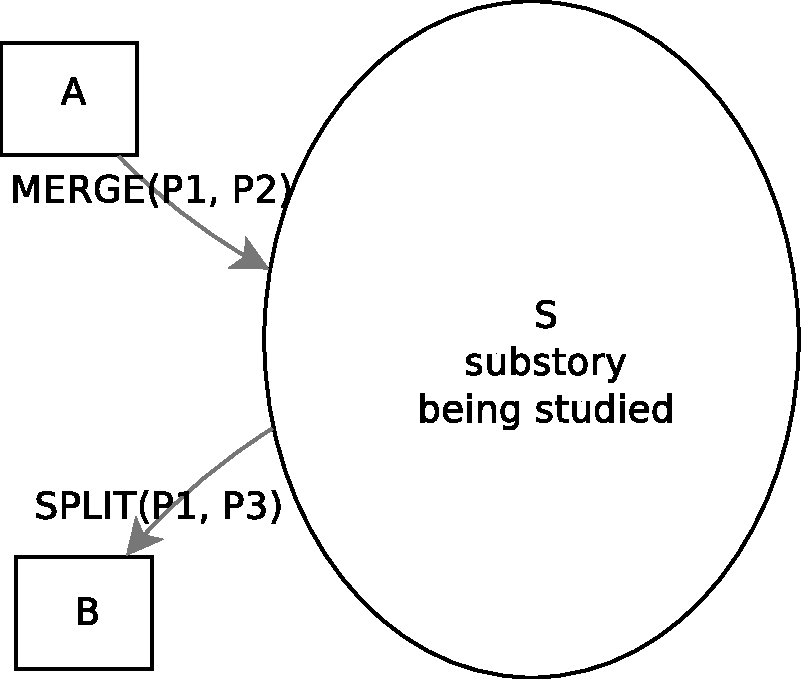
\includegraphics[scale=0.34]{figures/graph-4.pdf}
\label{fig:related-articles}
\end{center}
\end{figure}

\subsubsection{Queryability}
Our system is queryable by users, where a query entered by a user is in the form of filter on the actors and/or topics talked about in the
news corpus. Hence, the users need only to pick a suitable filter to study the intended story in desired detail. For eg., an example query could
be ``CORRUPTION AND ROBERT VADRA AND HARYANA'' which yields all stories around the corruption scandal involving Robert Vadra
(an Indian businessman) in Haryana (a state in India).
\subsubsection{Faceted Searchability}
Our system is a guided environment where a user is presented with popular actors, topics, events, time periods, etc automatically from the 
news corpus, which guide her search to discover and explore more popular stories first. These also serve to label different stories and guide the
user towards a more refined query around specific substories. Figure~\ref{fig:faceted-search} shows a snapshot of this feature.
\begin{figure}[ht]
\begin{center}
\caption{Analytics which help the user better understand the stories}
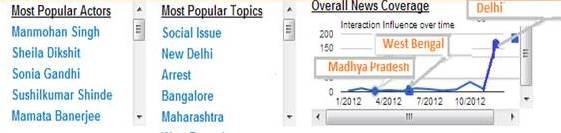
\includegraphics[scale=0.34]{figures/faceted.png}
\label{fig:faceted-search}
\end{center}
\end{figure}

\subsubsection{Structured storage of an article stream}
The rate at which new articles are published is growing exponentially. If a system
has to do well at taking in a live input stream of news articles, it can afford to process this set only once, and then store this set in a structure
which is efficient to maintain and query later. In most cases, this structure would come from the text content of the articles coming from a third-party media organization, 
but once derived, the text content need not be duplicated by the browsing system. The structure should be rich enough to answer all queries of the user, without
processing the article text again.
\subsubsection{On-demand detail}
The system should respect the user's final say in the detail at which different stories are visualized. Should the system
just give a 10-line summary of the event captured by 5 articles? Or should it focus in to the 5 articles, creating 2 sub-stories within them? This decision
should be left to the user as a preference.
\subsubsection{No Redundancy in the News stories}
News articles around a single story tend to summarize past events, so as to be give some 
context to the reader following this story. However, a browsing system should remove such redundancy, and summarize various facets of the story
that are developed in the sequence of articles, so that event appears once at the time of first reporting
\subsection{Block System Design}
\label{sec:block}

The strength of our approach is that we only need to process our input news article set only once. From the raw set of news articles, we
generate and store a graph representation formed by considering the most important transformations that are mined. We claim that this graphical 
representation of the article set is rich enough to answer different kinds of user queries. Having created a news graph from the news corpus, we showed how to meet the requirements of a good news browsing system.
Figure~\ref{fig:block-system-design} shows our block system design. It can be divided into
two major components - Offline and Online. The offline component handles incoming news articles, and augments them into our underlying graph data structure representation stored
in the database. The online component interfaces with the user, and based on the user's query, identifies the parts of the graph to visualize and 
shows the relevant stories. To further optimize, we need to only save the structure with pointers to web URL of the articles and query it only while presenting to the user. We will now briefly describe each aspect of our system.
\subsection{Preprocessing Steps}
\subsubsection*{News Corpus}
Our news corpus is a subset of articles from the Indian national daily {\em The Hindu}\footnote{http://thehindu.com}, across a variety of broad categories like Crime, Economy, Government, etc. 
{\em The Hindu} was chosen because it is a popular Indian daily, and offers a convenient way to download articles along with rich meta-data like Topic tags.
\subsubsection*{Entity Extraction}
We used the OpenCalais\footnote{http://opencalais.com} API to extract all the entities appearing in the articles. In particular, we call
the people featured in the articles as actors. We found the result of OpenCalais to be the most accurate among the NER tools we experimented with.
For sanitizing the mined entity set (correct spelling errors, remap aliases of the same entity to a unique identifier, remove ambiguous entity tokens),
we used an ontology(YAGO\footnote{http://www.mpi-inf.mpg.de/yago-naga/yago/}) based approach.
\subsubsection*{Topic Detection}
Along with the entities for an article, we also need the list of topics that were talked about in the article. 
We relied on the Hindu articles being hand tagged-at-source by rich and relevant Topic tags. These are much more expressive compared to an automated technique of topic detection.
\begin{figure}
\caption{Block system diagram of our News Browsing tool}
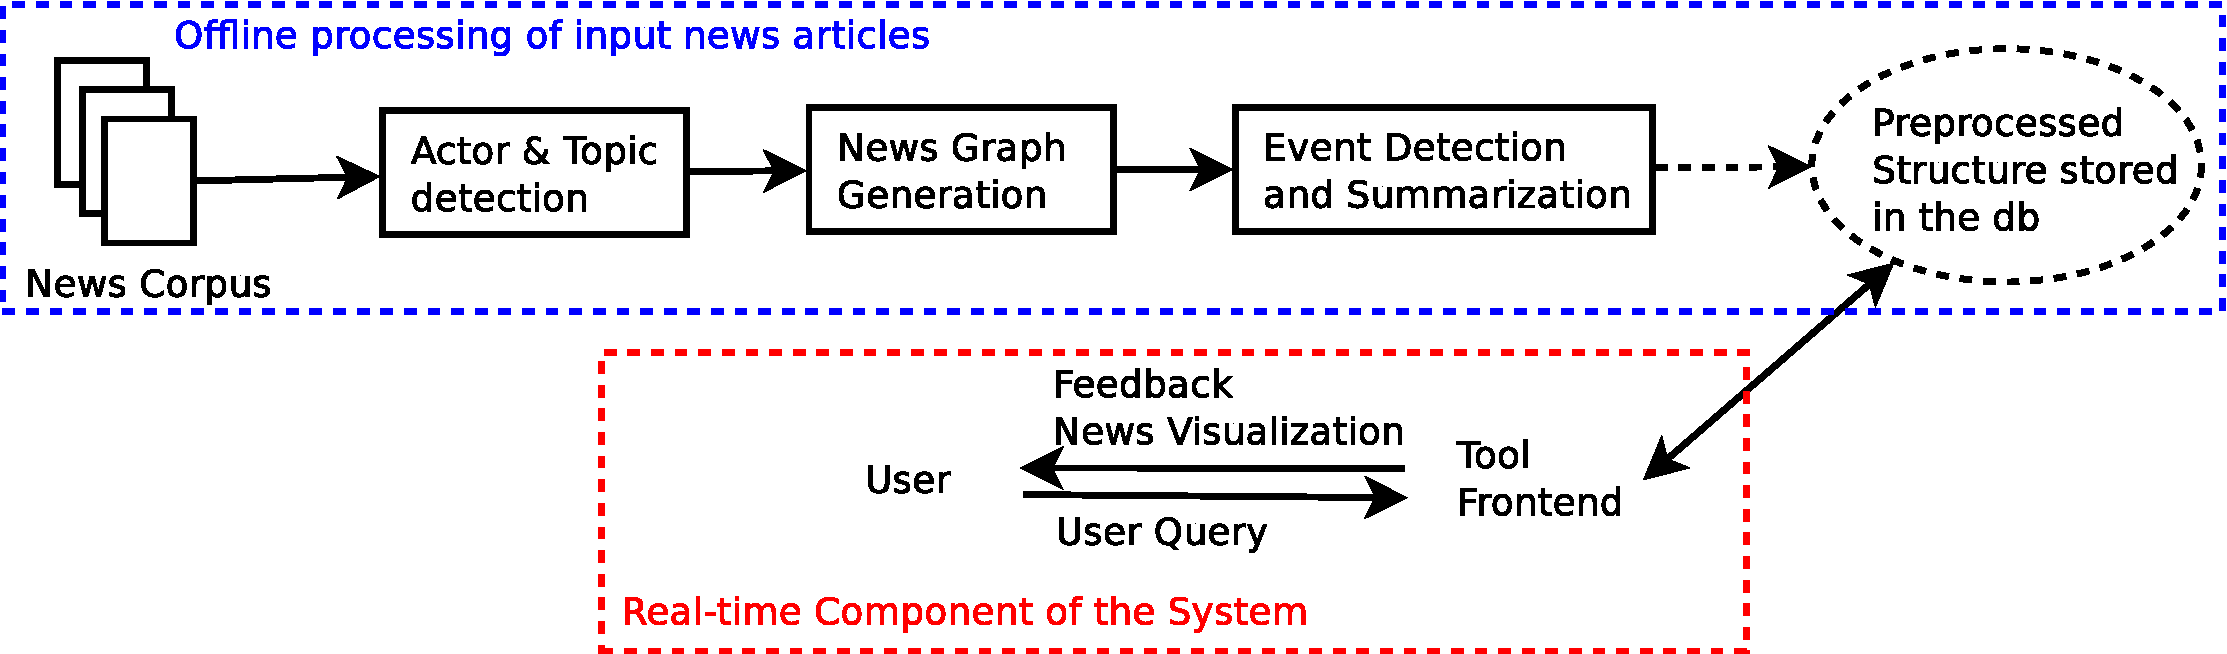
\includegraphics[scale=0.24]{figures/system-design.pdf}
\label{fig:block-system-design}
\end{figure}
\begin{figure*}
\caption{A graph snippet showing multiple stories}
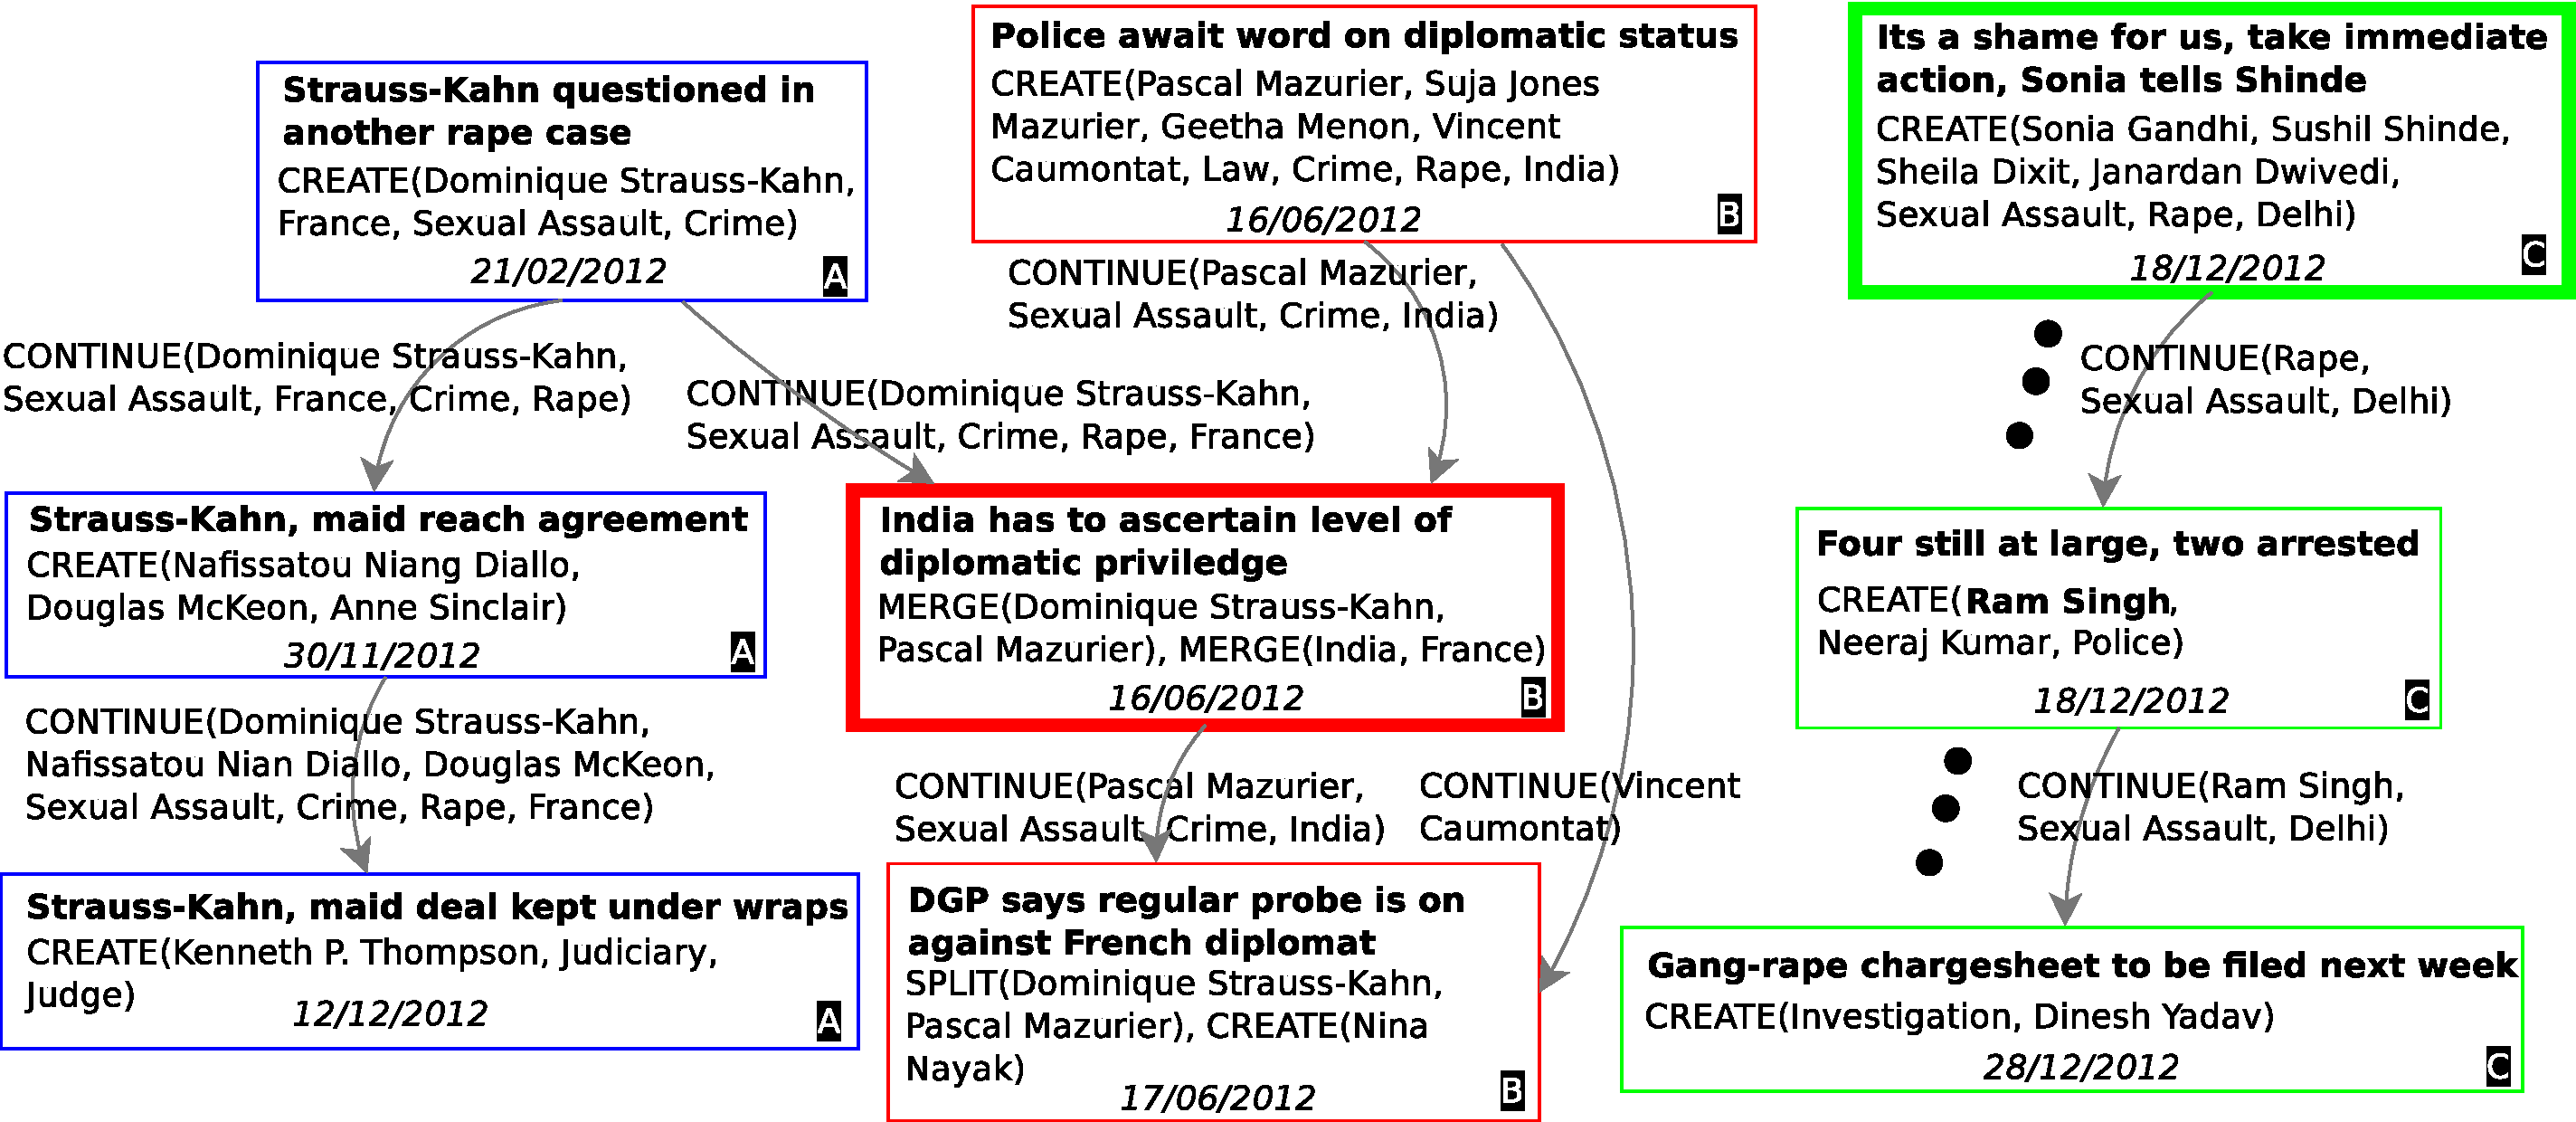
\includegraphics[scale=0.34]{figures/graph-2.pdf}
\label{fig:context-graph-example}
\end{figure*}

\subsection{News Graph Generation}\label{sec:graph-desc}
Our work implements and builds upon the work by Choudhary et
al.\cite{choudhary@ecir2008} which formalizes the notion of presenting
news articles as a directed graph.  Their algorithm can be extended to
augment new articles on to a pre-built graph since it considers
articles sequentially.  The following sequence of update steps are to
be followed on augmenting a new article $a_t$ published at $t$, into
the graph structure.
\begin{enumerate}
  \item Tag $a_t$ with relevant actors and topics
  \item Find all articles $A = a_\tau$ s.t. $\tau+F \leq t$.
  \item For the articles in the set $A$, mine all additional transformations that emerge
  \item Recompute the min-weight edge-covering locally in the subgraphs containing articles from $A$
  \item For the new article $a_t$, repeat the steps required for adding a new article into the graph
  \item Re-cluster the graph locally to determine to assign a cluster to the new node
\end{enumerate}
By taking the recommended values of the parameters, we were able to generate a news graph on 1000 nodes in around 4 minutes on a Dell Intel Centrino machine.
Adding newer articles to this graph was significantly cheaper, taking only around 10 seconds depending on the article size, etc.
Moreover, it only looks at articles within a time window, and hence different parts of the graph can be generated in parallel.

Figure~\ref{fig:sample-news-graph}  shows an example of a part of the graph created on articles that followed a Rape Case incident during February-April 2012. We see how the
story starts with the media covering initial case being filed and the police investigations.

\subsection{Event detection, summarization \& Context extraction}\label{sec:event-detection-summary-context}
\subsubsection*{Event detection}
We found the resultant graph from the previous step not suitable for visualization. The graph created is usally very dense, making it hard to follow and study a subgraph in isolation.
Every edge in the graph covers some transformations between articles, however to convey the purpose of every edge, one needs to label it with the transformations that the edge covers, 
which further makes visualization overwhelming. 
We consider this graph more suitable as a rich back-end.
This graph is created by pre-processing the news corpus once, and then a standard node clustering algorithm (Markov graph clustering) is applied to draw out clusters in this graph. 
These clusters are considered as events that happen in the corpus. Different clusters may or may not talk about the same story, depending on the proximity of the clusters.
In this way, an event is a cluster of the news graph, which may contain one or more articles. 
This graph is now useful for answering questions like detecting significant events (dense node clusters), developments in the life of a particular group of actors (visualizing the subgraphs 
involving the actor set), etc. The intuition behind how the graph structure relates to events in the real world is natural if we study how media reports events. 
For eg., consider an event like some criminal offence followed by a law suite. At first, articles which talk about the offence and alleged victims and culprits starts appearing. Then, this is gradually
replaced by the ongoing trial. Across these articles, the common threads are the topics and the CONTINUE/MERGE transformations among the actors (victims and culprits). Hence, these naturally form node clusters in the graph. This real world event is captured 
by the sequence of the articles that appeared.
As we show in Section~\ref{sec:baseline-comparison}, events determined by way of clustering on the graph is preferred by users to a similar clustering
done on raw articles in most cases.
\subsubsection*{Event summarization}
To make it easier for the user to understand an event, we summarize the articles of this event to give a broad idea of the event and show this summarization alongside the articles capturing that event (Section \ref{sec:filter-summarization}). For this, we tried out various document summarizing tools. We finally decided to Text Compactor \footnote{http://textcompactor.com/} which is based on Open Text Summarizer\footnote{http:/libots.sourceforge.net/} and has a convenient API. 
\subsubsection*{Context extraction}
Due to richness of the news graph, the neighbourhood of the story (subgraphs of the base news graph) being currently visualized, serves to add
useful context. Moreover, different parts of the neighbourhood model different transformations and hence, following
different neighbours amounts to adding a more unique kind of context, which gives a unique interpretation of the overall story. 
\subsection {Frontend interface}
Our interface is built on HTML using Javascript and PHP on the server-side, using TimelineJS\footnote{http://timeline.verite.co/} and Google Visualization API\footnote{http://developers.google.com/chart/interactive/docs/reference} libraries.
Figure~\ref{fig:complete-tool-screenshot} shows a screenshot of our webtool. The interface
has 3 primary parts: the Filtering \& feedback pane, the News article(s) \& summary pane and the Timeline pane. 
\subsubsection*{Filtering \& feedback pane}
Our system deeply analyzes the news corpus to mine all the featured actors and topics, and makes them queryable. The user selects one or more actors
and/or topics to filter news only about them. The user could also restrict on a particular time window. Relative to the filter parameters set by her, 
the user gets more context by way of getting a ranked list of ``Popular Actors'' and ``Popular Topics''. In addition, we also plot the number of
articles published against time to study what stories were popular at what times. 
\subsubsection*{Timeline pane}
Having selected suitable filters, the user is presented with all the different events detected from the graph on the timeline. These appear as 
bubbles on the timeline, with a start and end date. The user can easily move in time, skimming through uninteresting news events.
More popular events (as judged by the density of nodes \& edges in the cluster), are highlighted in yellow to guide the user.
On clicking a particular bubble, that event is highlighted and the corresponding story is shown in the middle pane. Figure~\ref{fig:timeline-closeup}
shows a snippet of the timeline, with each bubble an event (one or more articles) at some time, and the most significant bubble highlighted in yellow.
\begin{figure}
\caption{A screenshot of the timeline showing event bubbles}
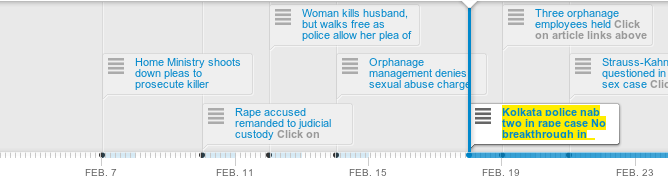
\includegraphics[scale=0.34]{figures/timeline2.png}
\label{fig:timeline-closeup}
\end{figure}
\subsubsection*{News articles \& summary pane}\label{sec:filter-summarization}
Having selected a particular story to focus on, the user can read all articles arranged sequentially so it is easy to read them in succession.
On the right, we show a summary generated from the articles of this story by the methods discussed in Section \ref{sec:event-detection-summary-context}.
On clicking an article, the user is served the full article text. The user is also shown the full list of actors and topics discussed in this story.

\section{Evaluation}
\label{sec:eval}

We conducted several user studies to evaluate ESTHETE, which is a system composed of a data structural graphical representation of news articles with a timeline-based visualisation.
 %%MR: I have talked specifically about presentation here. Make sure that this has been described somewhere in the text previously. 

\squishlist
	
	\item {\bf Usability and Effectiveness:} For our system to be useful, not only does it have to be easy to use, but also help users understand the big picture of the news story they are interested in. Our experiments in \ref{subsec:usability} evaluate these aspects.
	
	\item {\bf Precision:} A story presented on the timeline has several different aspects associated with it.  A user can filter out the relevant aspects by selecting or deselecting topics and actors identified by the system. When a user issues a filter query, how relevant are the returned results? Note that querying is not just a keyword match, but also computes and returns context-adding articles (Section~\ref{sec:finding-context}).
	
	\item {\bf News graphs as a framework:} Finally, our third experiment establishes the usefulness of representing news articles as a graph. We compare our news graph framework to two other baselines -- the articles themselves, and a clustering of articles using k-means clustering.
	
\squishend


\subsection{Setup}
Our news corpus consists of articles published by ``The Hindu'', a popular Indian newspaper. We choose three groups of articles corresponding to ``rape'', ``corruption'' and ``petrol price''. We fired each of these keywords into the website's search form and downloaded all articles that were returned. Therefore, we had three article groups corresponding to the three keywords. The total no. of articles is 10,121, published between 2010-2013. Each group had specific \emph{subsets} of articles corresponding to recent stories in the news. The first group of articles contained, in addition to articles about rape cases in various parts of India and abroad, articles about a gang-rape of a woman on a bus, which led to several weeks of protests in Delhi. Similarly, the second group of articles contained a ``sub-story'' about a very high-profile anti-corruption protest in Delhi, which then morphed into a political story about accusations of corruption against the son-in-law (Robert Vadra) of a powerful politician. The third group of articles contained a sub-story about petrol prices in the year 2012 which lead to political unrest. %%MR: I am not very familiar with this story, please check.

Each article group was then organised as a news graph using the techniques explained in Section \ref{sec:graph-desc}  %we need to mention this 
and the following three sub stories (described in the previous paragraph), were used for experimentation i) the gang-rape incident in Delhi (S1), ii) corruption stories related to Robert Vadra (S2), and, iii) petrol price (S3).

The three user studies made use of the following setup: an article group, in its entirety was presented to the user on our interface. The users were then allowed to interact with the system using whatever filters they felt would be useful. The focus of each set of experiments (described below) were the three sub stories.

%Each of the experiments made use of different kinds of users. For the first experiment of evaluating the precision of our system, we made use of people who had intimate knowledge of the three stories. For the next two experiments the users ranged from college-going students to expert journalists.

\subsection{Experiment design and results}

\subsubsection{Usability and Effectiveness}
\label{subsec:usability}
\begin{table}
\begin{center}
\small
%\hline
\begin{tabular}{|p{.69cm}|p{.65cm}|p{.70cm}|p{.70cm}|p{.70cm}|p{.70cm}|p{.70cm}|p{.70cm}|}
\hline
\multirow{2}{*}{{\bf Story}} & \multirow{2}{*}{\parbox{.55cm}{{\bf \# users}}} & \multicolumn{2}{p{1.85cm}|}{{\bf Ease of use}} & \multicolumn{2}{p{1.95cm}|}{\centering{\bf New Information}} & \multicolumn{2}{p{1.55cm}|}{\centering{\bf Big Picture}}\\ 
\cline{3-8} & & E & G & E & G & E & G \\
\hline
S1 & 22 & 3.76 & 4.25 & 4.25 & 3.4 & 4.3 & 3.66\\
S2 & 12 & 3.83 & 4.18 & 4.29 & 3.5 & 4.39 & 3.71 \\
S3 & 6 & 3.75 & 4.33 & 4.4 & 3.5 & 4.4 & 3.66\\
\hline
\hline
All & 40 & 3.78 & 4.24 & 4.28 & 3.44 & 4.34 & 3.67\\
\hline
\end{tabular}
\end{center}
\caption{Average ratings for usability (out of 5); E:ESTHETE, G: Google News}
\label{tab:ease}
\end{table}

\normalsize
\subsubsection*{Usability}
In order to evaluate the usability of ESTHETE, we asked 40 users to pick a story of their choice (among S1, S2 and S3) and to study that story by interacting with ESTHETE and Google News, in any order, for 15 minutes respectively. After the users had interacted with both the systems, we asked users the following questions:

\squishlist
	\item {\bf (Q1) Ease of use:} On a scale of 1 to 5, how would you rate both the systems on their ease of use (with 5 corresponding to ``very easy'')?
	\item {\bf (Q2) New Information:} Given your current knowledge of the story, how would you rate both the systems on their ability to provide new information that you weren't aware of before interacting with the systems? (1 corresponds to ``no new information'', 5 corresponds to ``more than satisfactory'')
	\item {\bf (Q3) Big Picture:} How would you rate both the systems on their ability to aid your understanding of the big picture of the story? (1 corresponds to ``not at all'', 5 corresponds to ``perfectly well'')
\squishend

The results are tabulated in Table \ref{tab:ease}.
Clearly, the users found our system to be more effective than Google News in gaining new information and understanding the bigger picture of the story, in a short time frame. This shows the ability of our system ESTHETE to bring forth and coherently link important nuggets of information. This also exhibits our system's ability to present the user with the necessary context that aided their understanding of the bigger picture of the story. The users also found the system easy to use and navigate.


%%MR: Instead of using ``tool'', use ``system''
\begin{table}
\small
\begin{tabular}{|c|p{7cm}|}
\hline
{\bf Story} & {\bf Questions asked}\\
\hline
S1 & {\em Did you learn about the reactions of different political particles to the Delhi rape incident?}, {\em Did you learn about the health condition of the victim following the crime?}\\
\hline
S2 & {\em Did you learn about the interactions between Arvind Kejriwal and Robert Vadra?}\\
\hline
S2 & {\em Did you learn about the reactions of AIDMK and DMK to the petrol price hike?}\\
\hline
\end{tabular}
\caption{Yes-No questions asked to compare ESTHETE with Google News}
\label{tab:domain-yes-no-questions}
\end{table}
\subsubsection*{Effectiveness}
We also compared the effectiveness of our system, to help users understand a story in depth, with Google News. We asked 18 users to use either our system or Google News in order to understand any of the three stories listed above. The users had to pick one story of their interest and were allowed to interact with their chosen system for a session lasting 25 minutes. The user's task was to learn as much as they can about their chosen story using a system. Then, once they had completed their
interaction with their chosen system (ESTHETE or Google News), they were asked to answer a series of very specific questions related to the story they studied. Some of these questions are shown in Table~\ref{tab:domain-yes-no-questions}. For these questions, the users had to answer a Yes or a No based on their perception of how easy or difficult they feel it is to answer these questions using the system they just used. The users replied Yes if they felt that they could answer the question using the system they just used and vice versa.

\begin{table}
\small
\begin{center}
\begin{tabular}{|l|p{1.00cm}|p{1.45cm}|p{1.00cm}|p{1.00cm}|p{1.00cm}|}
\hline
%% Rahul: I feel that the column headings of the table are a bit unclear.
{\bf Story} & {\bf \# responses} & {\bf ESTHETE only} & {\bf Google News only} & {\bf Both} &{\bf None}\\
\hline
S1 & 36 & 23 & 2 & 9 & 2\\
S2 & 12 & 9 & 0 & 2 & 1\\
S3 & 6 & 3 & 0 & 3 & 0 \\
\hline
\end{tabular}
\end{center}
\caption{Effectiveness of ESTHETE}
\label{tab:effectiveness}
\end{table}
\normalsize
The results are tabulated in Table \ref{tab:effectiveness}. The table entries shows for a particular story, the number of responses for which the users responded that they can answer the underlying question using only ESTHETE, only Google News, from both and from none of these systems. The results shows that users found it easier to answer the story-related questions using our system, in comparision to Google News. This clearly demonstrates that our system is more effective than Google News in aiding the users get enough information for answering the story-specific questions. This study brings out the ability of our system to improve the user's understanding of the underlying story.  

\subsubsection{Precision of the system}
\begin{table}
\begin{center}
\small
\begin{tabular}{|c|p{1.25cm}|p{1.25cm}|c|}
\hline
{\bf Story} & {\bf \# users} & {\bf Avg. \# filters} & {\bf Precision}\\
\hline
S1 & 10 & 3.4 & 0.89\\
S2 & 10 & 2.5 & 0.92\\
S3 & 8 & 2.1 & 0.88\\
\hline
\end{tabular}
\end{center}
\caption{Precision of articles returned by the system using filters}
\label{tab:prec}
\end{table}

\normalsize

\paragraph*{Description} In order to measure the precision of the system, users who had intimate knowledge of the three stories were shown the news graph for the entire timeline and allowed to filter these stories using whatever keywords they felt were appropriate from the list of entities and topics extracted by our system. For example, if they filtered on ``Robert Vadra'' (story S2), they would retain articles which not only contained ``Robert Vadra'', but also articles which had a strong connection to him in relation to the corruption allegations against him. The users than judged the relevance of each of these filtered articles on a 2-point scale (either relevant or not relevant). On average, for each story, users used 2-4 filters (that is, they judged the relevance for 2-4 subsets of articles within the larger timeline).

\paragraph*{Results} The results of this experiment are tabulated in Table \ref{tab:prec}. The precision values are in the range 88\%-92\%, indicating that our representation framework is very effective in identifying different contexts.

\eat{
%RG-RM: Some discussion on why the precision values are not 100%

On discussing their assessments with users, we identified two 

%% This first reason about context-adding articles is not quite convincing -- it's like blaming the user.. It might look like users were being very subjective in their assessments -- judging something as relevant only if they did not know about it, rather than ignoring what they know. I have commented both reasons out.
We feel that the precision of our system is not closer to the maximum value of 1 for a variety of reasons. %%MR: Extra discussion.
\begin{itemize}
  \item \textbf {Context-adding articles}: In the hope of adding more context to a user's news browsing experience, we also return articles which are not
  directly related to her input filters, but strongly related to the articles about $P$. However, if the user already has enough context and prior knowledge, 
  such articles become extraneous and are considered irrelevant. For eg., consider a corruption scandal, where a politician $P$ becomes the prime accused
  after a few months of investigation. In such a case, filtering on $P$ also returns articles talking about this case, but not explicitly mentioning $P$.
  For a user with enough prior knowledge of the case, such information is not relevant since she wanted to understand the specific involvement of $P$.
  \item \textbf {Inter-annotator disagreement}: There were cases where two differrent annotators marked the same article as relevant and irrelevant
  respectively on the same task. %%MR: It is no longer ``task'', right? It is the filter. In that case, you should ensure that there are at least 3 annotators and take the majority. Is this the case? If not, I would rather just leave this out.
\end{itemize}
}

\subsubsection{News graphs as a framework}\label{sec:baseline-comparison}
\begin{table}
\begin{center}
\small
\begin{tabular}{|l|p{1cm}|p{1.5cm}|p{1.5cm}|p{1.5cm}|}
\hline
{\bf Story} & {\bf No. of users} & {\bf ESTHETE preferred} & {\bf B1 preferred} & {\bf B2 preferred}\\
\hline
S1 & 7 & 100\% & 0\% & 0\%\\
S2 & 6 & 83\% & 0\% & 17\%\\
S3 & 7 & 100\% & 0\% & 0\%\\
\hline
\end{tabular}
\end{center}
\caption{Comparison of news graphs against baselines B1 and B2} %%MR: Need to change
\label{tab:graph}
\end{table}

\normalsize

\paragraph*{Description} In order to determine how news graphs compare against other ways of representing news corpora, we designed the following two baselines, both of which also made use of our timeline interface. Our first baseline (B1) simply presents \emph{all} articles (corresponding to the article groups mentioned above) on the timeline according to date of publication. For our second baseline (B2), we clustered each article group using k-means clustering, and then presented these clusters on our timeline. Therefore, visually, all three techniques looked the same. Three timelines corresponding to the three techniques were then simultaneously presented to the user and the user was asked to pick the one that they preferred in terms of understanding the various stories.

 %Clearly, our representation was preferred. %%MR: Note that we are talking about ``our clustering'' vs. ``k-means''. Make sure that this point is brought out in the text previously -- that news graph representation is a means of clustering. Otherwise these lines have no meaning.
\paragraph*{Results} The results of this experiment are tabulated in Table \ref{tab:graph}. For all 3 article groups, our representation is preferred over the other two baselines. This implies that not only is the quality of the clusters formed by our technique better than k-means, but also that the context we provide to the users is actually found to be beneficial. For the story $S2$, $B2$ was preferred by 1 user because of the time-localised characteristic of the story $S2$, due to which that user couldn't benefit from the context added by our system.


%%MR: Any explanation as to why B2 was preferred for story 2?


%\section{Acknowledgments}
We would like to thank all users who agreed to do our survey and rate our system. 
%In particular, we would like to thank Dr. Parag Singla, Pranay Agarwal, Ashwin Venkataraman and Varun Malhotra for their help. 

\section{Conclusions}
\label{sec:conclusions}

The main contribution of this paper is the formalization of a natural
notion, personalized flexible context extraction, that corresponds to
a need that all news consumers have felt to some extent or the
other. We have outlined the structure of a system that is geared to
provide a richly featured news browsing experience that revolves
around the notion of context. Using the news graphs first described by
Choudhary et. al.~\cite{choudhary@ecir2008} we have shown how such a
news browsing experience can be achieved. Our news browsing tool,
ESTHETE, attempts to provide the kind of context-aware news
consumption environment that makes it possible for a lay user, or an
expert, to explore the various aspects of a story to whatever level of
detail required, and does not tie down the user to particular
structures extracted from the corpus. The fundamental difference
between this work and the literature preceding it is that earlier
papers took the approach of developing algorithms for processing the
corpus to respond to certain classes of queries whereas we approach
news browsing as a data structuring problem, preprocessing the corpus
into a structured entity that contains the complex relations that a
human being needs to unravel the context of a particular news
story. Our user studies have shown that ESTHETE addresses the need for
context without sacrficing on the need for current information and
overall provides complex features in an easy-to-use interface.



\bibliographystyle{abbrv}
\bibliography{news}  % news.bib is the name of the Bibliography in this case


\end{document}
